%\chapter{Design of a SNP genotyping array specific to the African continent}
\section{Simulated and preliminary design of a SNP genotyping array specific to the African continent}
\label{sec:chip_design}
\chapter{Design of a SNP array specific to the African continent}
\label{ch:chip_design}

\section{Introduction}
As shown in table \ref{tab:chip_SNPs} on \pageref{tab:chip_SNPs), figure \ref{fig:SN02f2} and elsewhere\cite{Gurdasani2015} approximately 20\% of the autosomal SNPs on the Illumina HumanOmni2.5 SNP array are monomorphic in African populations. And as shown in figure \ref{fig:SN10f2} on page \pageref{fig:SN10f2} SNP density also alters imputation accuracy quite significantly. Therefore we wish to explore whether a continent specific array can capture variation in African populations better.

\begin{figure}
\centering
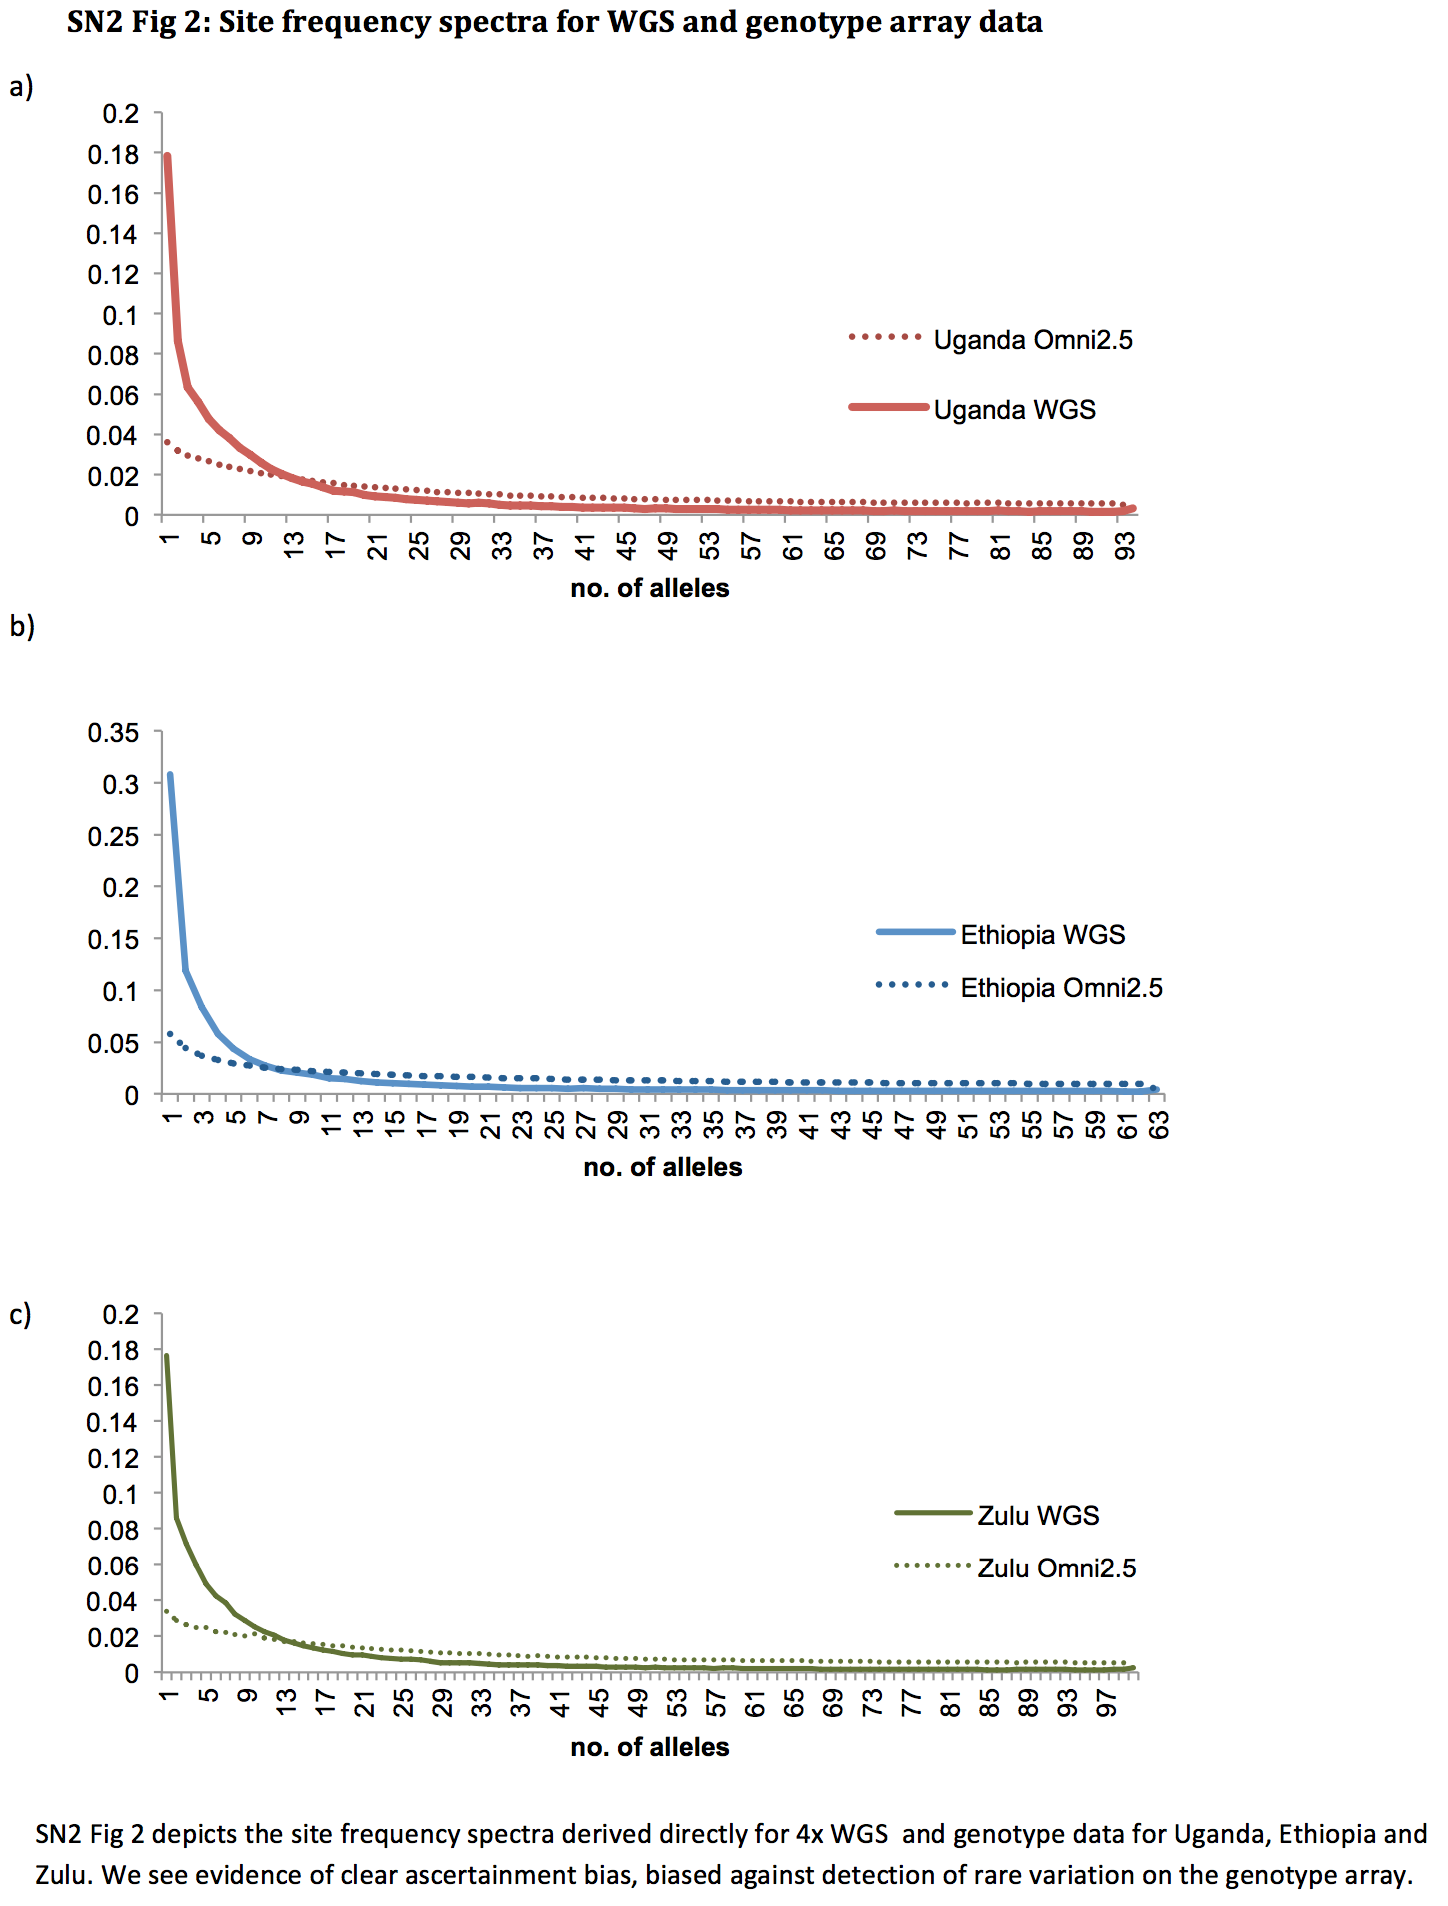
\includegraphics[trim={0 2cm 4cm 1cm},clip,width=0.8\textwidth]{fig/SN02f2}
\caption[Site frequency spectrum of sequence and SNP array data]{Site frequency spectrum derived directly from 4x \gls{WGS} data and SNP array data for the populations Uganda, Zulu and Ethiopia. Ascertainment bias against detection of rare variation on the SNP array is seen. On the x-axis is the number of alleles. On the y-axis is the relative frequency for each allele count.}
\label{fig:SN02f2}
\end{figure}

\section{Data description}
\section{Methods}
Haplotype files are block gzipped\cite{Li05012011}, which allows them to be indexed. This allows for rapid calculation of pairwise \gls{LD} between \glspl{SNP} in a window of a certain size with a small amount of memory usage. I calculated the LD with Python3\footnote{https://github.com/team149/tc9/blob/master/ragtagger/calculateLD.py}. Alternatively the pairwise \gls{LD} values can now be calculated with PLINK1.9\cite{25722852}. These pairwise LD values are then used as input for the tag SNP selection program RagTagger\footnote{https://github.com/team149/tc9/blob/master/ragtagger/ragtagger.py}.

\subsection{Selection of tag SNPs and identification of informative variants for a hypothetical SNP array}
\begin{figure}[htp]
\centering
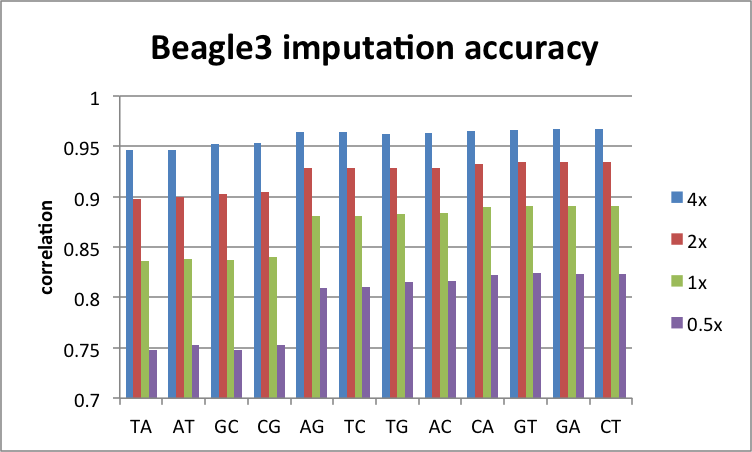
\includegraphics{Chapter3/fig/imp_accu_allele}
\caption{Imputation accuracy for each heterzygous allele. We used the Baganda 4x sequence data and SNP array data to calculate the genotype correlation for each heterozygous allele type. We found that the "mirror" alleles AT/TA and CG/GC for which it can be difficult to determine the relative strand have lower genotype correlations. }
\label{fig:imp_accu_allele}
\end{figure}

For identification of informative variants on the chip array we utilised a hybrid algorithm with cycles of LD based pairwise tagging, and imputation, as previously described.\cite{Hoffmann2011422}

We have developed a multi-population tagging algorithm based on the algorithm TAGster for WGS data.\cite{Xu2007} The methods we used for tagging were identical to those used by TAGster; however, by using seeking and indexing approaches we were able to optimise the computational efficiency of the algorithm by an order of magnitude (unpublished data, Carstensen et al.). We briefly outline the tagging algorithm as follows (Figure 2):

\begin{enumerate}
\item Calculate LD (\textit{r}\textsuperscript{2}) between each SNP and all other SNPs in the flanking 250 KB region for each population separately. MAF thresholds are imposed at this stage, and only pairs of SNPs where both exceed the MAF threshold are included.
\item For each SNP not already in the tagging set, a count of SNPs in the target set that are in LD exceeding a given threshold \textit{r}\textsuperscript{2} with it is generated across the genome and summed across all populations.
\item The most informative SNP (the SNP with most target SNPs in LD with it summed across population) is chosen as the tagging SNP and added to the set of tagging SNPs. If two SNPs have the same ranking, then a SNP is chosen by one or all of the following parameters in order of preference: 1) presence on existing SNP arrays (count), 2) presence in 1000G and/or dbSNP (binary), 3) location within a gene region (binary), 4) binned genotyping score provided by the vendor, 5) rate of heterozygosity across all populations (continuous).
%We do not take the vicinity to existing tag SNPs into account, despite  SNPs in close proximity being able to interfere with each other when assayed.\cite{21535878} We expect the algorithm to avoid this problem, because SNPs in proximity of each other are also likely to be in LD with each other.
\item This tagging SNP and SNPs in LD with it are now removed from the set of target SNPs. This process is carried out separately for each population, so that a separate set of target SNPs is maintained for each population set. However, SNPs in LD with the tagging SNP can still be picked up as tagging SNPs themselves if they independently tag the maximum no. of SNPs in any iteration.
Steps 2-3 are repeated until either a specified number of SNPs or all target SNPs (chosen as SNPs above a specific MAF threshold per-population) are tagged across all population sets, or until a specific number of SNPs is reached, as specified.
\end{enumerate}

Although this method works well across populations, it only carries out pairwise single-marker tagging. Haplotype based, or multi-marker tagging would potentially be more efficient, and select fewer tagging sites. In order to incorporate haplotype based tagging into our model, we use a hybrid method, with cycles of tagging and imputation, as has been described before.\cite{Hoffmann2011422}

\begin{figure}
\centering
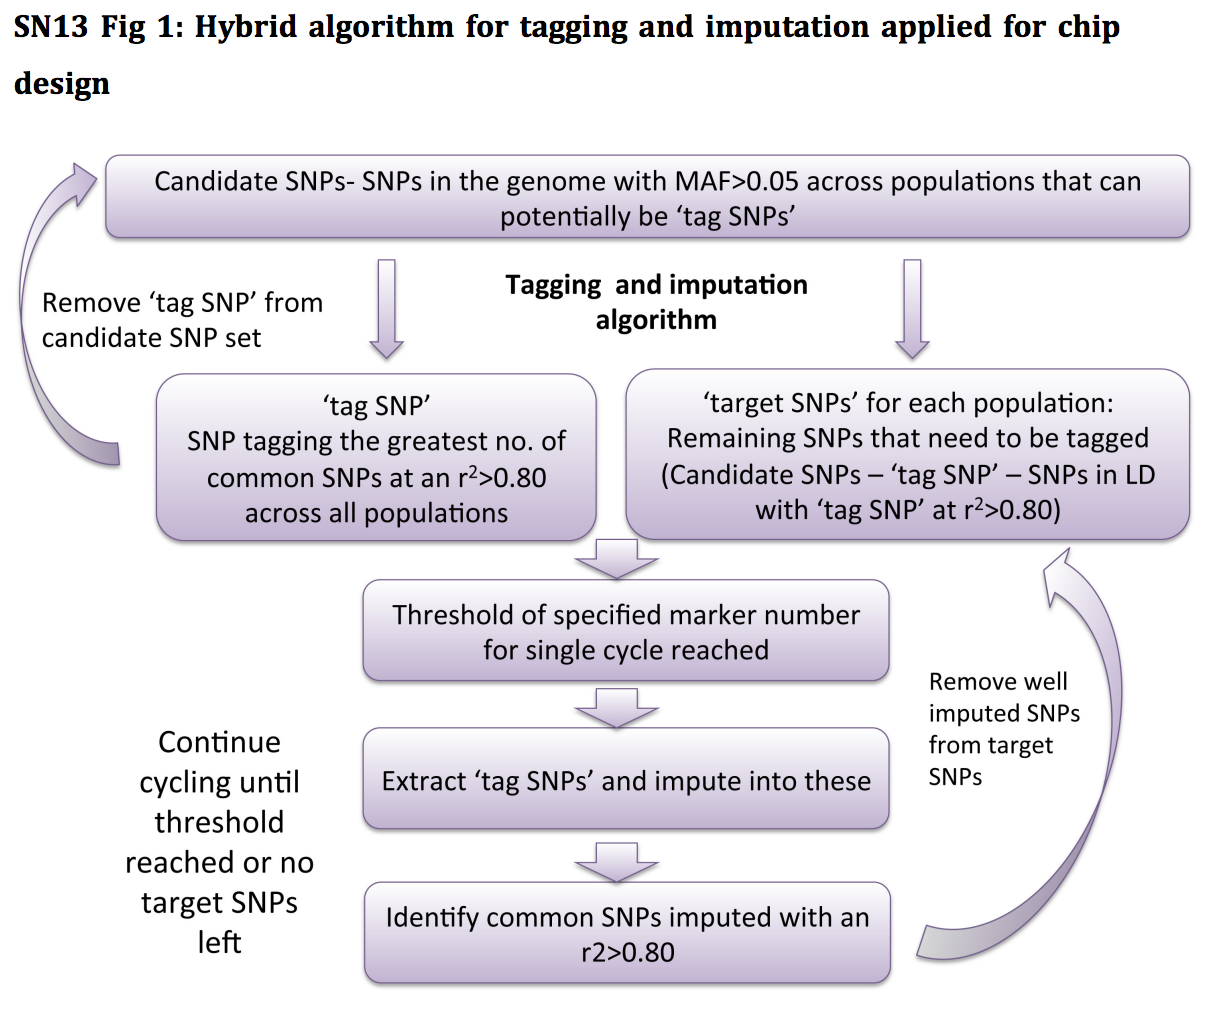
\includegraphics[trim={0 0 0 1cm},clip,width=0.75\textwidth]{fig/SN13f1}
\caption[xxx]{XXXXXXXX.}
\label{fig:SN13f1}
\end{figure}

We implement this method by selecting a maximum number of pre-defined tagging SNPs in the first cycle. With these tagging SNPs we simulate a chip for each population, and imputation is carried out using a reference panel, to identify additional sites in each population that are tagged at an $r^{2}$ threshold above 0.80 by the tagging sites. These sites are removed from the target set for each population, and do not contribute to the next cycle, thereby making the process more efficient. To maximise imputation accuracy we use all samples in table \ref{tab:samples} for the reference panel and merge this reference panel with haplotypes from all of the 1000G samples from Europe, Asia and the Americas not already present in the reference panel. However, for imputation into each population, all samples from the given population are removed from the reference panel. This ‘leave one population out’ approach would produce relatively conservative results for tagging, with more variants being tagged than if a subsample of the population was included in the reference panel. This is a more realistic scenario, as it is not necessary that any given population genotyped on the chip in future would be represented in the reference panel.

Additionally, pre-selected known biologically relevant variants, valuable to the studies planned for consortia can be included on the array, to replace certain tag SNPs. We have previously shown that a 1M tagging variants chosen using the described algorithm can produce \textgreater80\% coverage across diverse populations in Africa. Based on this, we plan to carry out approximately 10 cycles to capture 1.2M tagging variants, in order to prioritise variants to include in the design of a 1M chip array. Following this, we will further validate our tagging algorithm among populations with smaller sample sizes that were not included in the development in the chip array, by selecting tagging variants among these and imputing with the reference panel, excluding these populations. We estimate coverage of each population by such a chip array using imputation. Coverage is defined as the proportion of common variation captured at a correlation greater than 0.80 across the genome in a given population with the combined reference panel (excluding the population being evaluated). $r^{2}$, here, is calculated as the correlation between the sequence data and imputed data on a hypothetical 1M chip array for common variation. 

%Instead of random choice do 1) chip overlap, 2) quality score (VQSLOD and MVNcall posterior), 3) white/black list


\section{Results}

\subsection{Comparison of RagTagger with existing methods}
RagTagger uses less than 1GB of memory when selecting tag SNPs from a 2\gls{Mbp} fragment and runs to completion in a few minutes. TAGster\cite{Xu2007} uses more than 10GB of memory (16.5GB) on the same 2\gls{Mbp} fragment and takes longer than a day to run to completion (1.18 days). TAGster fails to run to completion when run across the whole genome and RagTagger finishes in 3 hours using less than 10GB of memory.

\subsection{Comparison of the Simple Greedy Algorithm and the Hybrid Algorithm}


\section{Discussion}
If more time and additional sequencing data had been available at the time of analysis, then it would have been interesting to compare the imputation accuracy, when using the Omni2.5M SNPs and the 1 million selected tag SNPs as an imputation scaffold. Given the large number of monomorphic SNPs on the Omni2.5M array and the European ascertainment bias, then it is expected, that the 1 million continent specific tag SNPs might perform better in terms of imputation accuracy.

\section{Conclusions}
The LD structure is different between continents. The selection of tag SNPs, which can best capture this alternate LD pattern, is important for increasing the ability to correctly estimate genotype probabilities of vicinal SNPs, which will for example lead to increased power in down-stream \glspl{GWAS}.